%
% pareto.tex
%
\renewcommand{\thisname}{Chart::Pareto}
\section{\thisname}
\name{\thisname}
\file{Pareto.pm}
\requires{Chart::Base, GD, Carp, FileHandle}
\begin{Description}
The class \thisclass creates a Pareto chart, \ie, a set of absolute
values overlaid with a line chart of the accumulated values. (This
latter curve is also known as an \emph{empirical cumulative distribution
function} or as a \emph{Lorenz curve}.) This representation usually
makes sense only if the values are sorted (either in ascending or in
descending order). \thisclass plots only one data set and its labels.
\thisclass is a subclass of \class{Chart::Base}.
\end{Description}

\example

\begin{figure}[ht]
  \begin{center}
    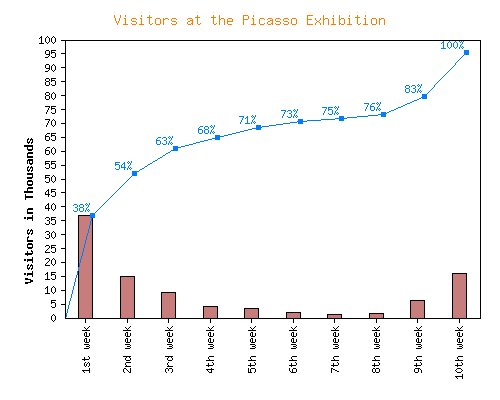
\includegraphics[scale=0.7]{d_pareto2.png}
  \end{center}
  \caption{Pareto chart}
  \label{fig:pareto}
\end{figure}
\begin{verbatim}
use Chart::Pareto;

$g = Chart::Pareto->new(500,400);
$g->add_dataset('1st week', '2nd week', '3rd week', '4th week',
                '5th week', '6th week', '7th week', '8th week',
                '9th week', '10th week');
$g->add_dataset(37, 15, 9, 4, 3.5, 2.1, 1.2, 1.5, 6.2, 16);

%hash = ('colors' => { 'dataset0' => 'mauve',
                       'dataset1' => 'light_blue',
                       'title' => 'orange'
                     },
         'title'              => 'Visitors at the Picasso Exhibition',
         'integer_ticks_only' => 'true',
         'skip_int_ticks'     => 5,
         'grey_background'    => 'false',
         'max_val'            => 100,
         'y_label'            => 'Visitors in Thousands',
         'x_ticks'            => 'vertical',
         'spaced_bars'        => 'true',
         'legend'             => 'none'
        );

$g->set(%hash);

$g->png("pareto.png");
\end{verbatim}

\constructorblurb{\thisname}

\begin{AttrDecl}{sort}
Sorts the data in ascending order if set to \literal{true}. Should be set if
the input data is not sorted. Defaults to \literal{false}.
\end{AttrDecl}

\begin{AttrDecl}{spaced\_bars}
Leaves some space between each group of bars when set to \literal{true}. This
usually make it easier to read a bar chart. Default is \literal{true}.
\end{AttrDecl}

\begin{AttrDecl}{y\_axes}
Tells \thisclass where to place the $y$ axis. Valid
values are \literal{left}, \literal{right} and \literal{both}. Defaults
to \literal{left}.
\end{AttrDecl}
